%  !TeX  root  =  user_guide.tex
\chapter{Les données OGC}\label{working_with_ogc}

% when the revision of a section has been finalized, 
% comment out the following line:
%\updatedisclaimer

% \qg supports WMS and WFS as data sources. WMS-support is native; WFS and WFS-T is
% implemented as a plugin.
\qg gère le WMS et le WFS comme source de données. La gestion du WMS est native tandis que les services WFS et WFS-T est géré sous forme d'extension.

% \section{What is OGC Data}\index{OGC!introduction}
\section{Qu'est-ce que les données OGC}\index{OGC!introduction}

%The Open Geospatial Consortium (OGC), is an international organization with more than 300 
%commercial, governmental, nonprofit and research organisations worldwide. Its members 
%develop and implement standards for geospatial content and services, GIS data processing 
%and exchange.
Le Consortium Geospatial Ouvert (Open Geospatial Consortium - OGC) est une organisation internationale à laquelle participent plus de 300 organisations commerciale, gouvernementale, associative et laboratoire de recherche à travers  le monde. Ses membres développent et implémentent des standards pour les services et le contenu géospatial, traitement de données SIG et de format d'échange.

%Describing a basic data model for geographic features an increasing number of specifications 
%are developed to serve specific needs for interoperable location and geospatial technology, 
%including GIS. Further information can be found under \url{http://www.opengeospatial.org/}.

%An increasing number of specifications describing a basic data model for
%geographic features are developed to serve specific needs for
%interoperable location and geospatial technology,  including GIS.
Un nombre croissant de spécifications décrivant une modélisation de donnée basique pour les objets géographiques ont été développées pour servir des besoins spécifiques dans des situations nécessitant une interopérabilité et des technologies géospatiales, dont les SIG. Des informations supplémentaires peuvent être trouvées sur le site
\url{http://www.opengeospatial.org/}.

% Important OGC specifications are:
Les spécifications importantes de l'OGC sont :

\begin{description}
\item[WMS :] Web Map Service
\item[WFS :] Web Feature Service
\item[WCS :] Web Coverage Service
\item[CAT :] Web Catalog Service
\item[SFS :] Simple Features for SQL
\item[GML :] Geography Markup Language
\end{description}

% OGC services are increasingly being used to exchange geospatial data between
% different GIS implementations and data stores. \qg can now deal with three of
% the above specifications, being SFS (though support of the PostgreSQL / PostGIS
% data provider, see Section \ref{label_postgis}); WFS and WMS as a client.
Les services OGC sont de plus en plus utilisés pour échanger des données géospatiales entre différentes implémentations SIG et des fournisseurs de données. \qg peut maintenant traiter trois des spécifications citées, ceux-ci étant SFS (par la gestion du fournisseur de données \ppg, voir section \ref{label_postgis}), comme client WFS et WMS.

\section{Client WMS}\label{sec:ogc-wms}\index{WMS!client}\index{OGC!WMS!client}\index{rasters!WMS}

\subsection{Aperçu de la gestion WMS}\label{sec:ogc-wms-about}\index{WMS!client!about}

% \qg currently can act as a WMS client that understands WMS 1.1, 1.1.1 and 1.3
% servers.  It has particularly been tested against publicly accessible servers
% such as DEMIS and JPL OnEarth.
\qg peut actuellement agir comme client WMS et comprend les versions 1.1, 1.1.1 et 1.3 des serveurs WMS. Il a été particulièrement testé avec des serveurs accessibles publiquement comme ceux de DEMIS et JPL OnEarth.

% WMS servers act upon requests by the client (e.g. \qg) for a raster map with
% a given extent, set of layers, symbolisation style, and transparency.  The WMS
% server then consults its local data sources, rasterizes the map, and sends
% it back to the client in a raster format.  For \qg this would typically
% be JPEG or PNG.
Les serveurs WMS agissent en fonction des requêtes envoyées par le client (par exemple \qg) pour une carte raster avec une étendue donnée, un ensemble de couches, une sémiologie et une transparence. Le serveur WMS consulte alors ses sources de données locales, rasterise la carte et la renvoie au client dans un format raster. Pour \qg, cela sera par exemple du JPEG ou du PNG.

%WMS is generically a REST (Representational State Transfer) service rather than
%a fully-blown Web Service.  As such, you can actually take the URLs generated by
%\qg and use them in a web browser to retrieve the same images that \qg uses
%internally.  This can be useful for troubleshooting, as there are
%several brands of WMS servers in the market and they all have their own
%interpretation of the WMS standard.
Un WMS est de manière générale un service web mis en oeuvre selon une architecture REST (Representational State Transfer) plutôt qu'un service RPC (Remote Procedure Call) pleinement déployé. De cette façon, vous pouvez copier les adresses générées par \qg et les copier dans un navigateur internet pou retrouver les mêmes images qu'utilise \qg. Cela peut être très pratique pour résoudre des problèmes, car de fait il y a plusieurs serveurs WMS existants ayant chacun une interprétation du standard WMS.

% WMS layers can be added quite simply, as long as you know the URL to access
% the WMS server, you have a serviceable connection to that server, and the
% server understands HTTP as the data transport mechanism.
Des couches WMS peuvent être ajoutées assez simplement, du moment que vous connaissez l'URL pour accéder au serveur WMS, vous avez une connexion sous forme de service sur ce serveur, et celui-ci comprend le protocole HTTP comme mécanisme de transport.

\subsection{Sélectionner des serveurs WMS}\label{sec:ogc-wms-servers}\index{WMS!remote server!selection}

% The first time you use the WMS feature, there are no servers defined. You 
% can begin by clicking the \toolbtntwo{mActionAddWmsLayer}{Add WMS layer}
% button inside the toolbar, or through the
% \mainmenuopt{Layer}>\dropmenuopttwo{mActionAddWmsLayer}{Add WMS Layer...}
% menu.
La première fois que vous utilisez la fonctionnalité des services WMS, il y a aucun serveur définie. Vous pouvez commencer en cliquant sur le bouton \toolbtntwo{mActionAddWmsLayer}{Ajoutez une couche WMS} dans la barre des outils ou à travers le menu \mainmenuopt{Couche}>\dropmenuopttwo{mActionAddWmsLayer}{Ajoutez une couche WMS\dots}

% The dialog \dialog{Add Layer(s) from a Server} for adding layers from the WMS
% server pops up. Fortunately you can add some servers to play with by clicking
% the \button{Add default servers} button. This will add at least three WMS
% servers for you to use, including the NASA (JPL) 
% WMS server. To define a new WMS server in the \tab{Server Connections}
% section, select \button{New}. Then enter in the parameters to connect to your
% desired WMS server, as listed in table \ref{tab:wms_connection_parms}:
La boîte de dialogue \dialog{Ajouter une couche d'un serveur} pour ajouter des couches d'un serveur WMS s'ouvre. Heureusement, vous pouvez ajouter des serveurs pour jouer en cliquant le bouton \button{Ajouter les serveurs par défaut}. Cela ajoutera au moins trois serveurs WMS pour tester, incluant celui de la NASA (JPL). Pour définir un nouveau serveur WMS dans la section \tab{Connexions au serveur}, sélectionnez \button{Nouveau}. Puis entrez les paramètres de connexion de votre serveur WMS désiré, comme listé dans le tableau \ref{tab:wms_connection_parms}:

\begin{table}[ht]\index{WMS!client!connection parameters}
\centering
% \caption{WMS Connection Parameters}\label{tab:wms_connection_parms}\medskip
 \begin{tabular}{|l|p{11cm}|}
% \hline Name & A name for this connection.  This name will be used in the
%  Server Connections drop-down box so that you can distinguish it from
%  other WMS Servers. \\
\hline Nom & Un nom pour cette connexion. Ce nom sera utilisé dans la liste déroulante des connexions aux serveurs afin que vous puissiez distinguer
des autres serveurs WMS. \\
% \hline URL \index{WMS!URL} & URL of the server providing the data.
%  This must be a resolvable host name; the same format as you would use 
%  to open a telnet connection or ping a host. \\
\hline URL \index{WMS!URL} & URL du serveur fournissant les données. Cela doit
être un nom d'hôte publique ; de même format que vous utilisez pour ouvrir une
connexion Telnet ou pinguer un hôte (ou dans un navigateur Internet). \\
\hline Nom utilisateur \index{WMS!authentification} & nom utilisateur pour accéder
à un serveur WMS sécurisé. Ce paramètre est optionnel \\
\hline Mot de passe & Mot de passe pour une authentification basique à un serveur 
WMS. Ce paramètre est optional.\\
\hline Ignorer l'adresse GetMap signalée & \checkbox{Ignorer l'adresse GetMap signalée}, utiliser l'URL définie au-dessus\\
\hline Ignorer l'adresse GetFeatureInfo signalée & \checkbox{Ignorer l'adresse GetFeatureInfo signalée}, utiliser l'URL définie au-dessus\\
\hline
\end{tabular}
\caption{Paramètres de connexion WMS}\label{tab:wms_connection_parms}
\end{table}

% If you need to set up a proxy-server to be able to receive WMS-services
% from the internet, you can add your proxy-server in the options.
% Choose menu \mainmenuopt{Settings} > \dropmenuopttwo{mActionOptions}{Options}
% and click on the \tab{Proxy} tab. There you can add your proxy-settings 
% and enable them by setting the \checkbox{Use proxy for web access}.
Si vous devez configurer un serveur proxy pour pouvoir recevoir des services WMS à partir d'Internet, vous pouvez ajouter votre serveur proxy dans les options. Choisissez le menu \mainmenuopt{Préférences} > \dropmenuopttwo{mActionOptions}{Options\dots} et cliquez sur l'onglet \tab{Proxy}. Vous pouvez alors ajouter votre configuration du proxy et l'activer en cochant la case \checkbox{Utiliser un proxy pour l'accès Internet} Assurez-vous que vous avez sélectionné le type de proxy correct dans la liste  déroulante\\ \dropmenuopt{Type de proxy}.

% Once the new WMS Server connection has been created, it will be 
% preserved for future \qg sessions.
Une fois que la nouvelle connexion du serveur WMS a été créée, elle sera sauvegardée pour les futures sessions de \qg.

% \begin{Tip}[ht]\caption{\textsc{On WMS Server URLs}}
% \qgistip{Be sure, when entering in the WMS server URL, that you have
% the base URL.  For example, you shouldn't have fragments such as
% \usertext{request=GetCapabilities} or \usertext{version=1.0.0}
% in your URL.\index{WMS!serveur distant!URL}
\begin{Tip}[ht]\caption{\textsc{À propos des URL des serveurs WMS}}
Assurez-vous, lorsque vous entrez l'URL du serveur WMS, d'avoir le début de l'URL. Par exemple, vous ne devez pas avoir ce genre de paramètre  \usertext{request=GetCapabilities} ou \usertext{version=1.0.0} dans votre URL\index{WMS!serveur distant!URL}
\end{Tip}

\subsection{Charger des couches WMS}\label{sec:ogc-wms-layers}\index{WMS!client!couches}

% Once you have successfully filled in your parameters you can select the
% \button{Connect} button to retrieve the capabilities of the selected server. 
% This includes the Image encoding, Layers, Layer Styles, and Projections. 
% Since this is a network operation, the speed of the response depends on the
% quality of your network connection to the WMS server. While downloading data
% from the WMS server, the download progress is visualized in the left bottom of
% the WMS Plugin dialog.
Une fois que vous avez rempli correctement vos paramètres, vous pouvez sélectionner le bouton \button{Se connecter} pour récupérer les possibilités du serveur sélectionné. Cela inclut le format d'image, les couches, les styles des couches et les projections. Puisque c'est une opération sur un réseau, la vitesse de la réponse dépend de la qualité de votre connexion réseau au serveur WMS. Pendant le téléchargement des données du serveur WMS, la progression du téléchargement est visualisée en bas à gauche de la boîte de dialogue de l'extension WMS.

% Your screen should now look a bit like Figure \ref{fig:connection_wms}, which
% shows the response provided by the NASA JPL OnEarth WMS server.
Votre écran doit ressembler un peu plus à la figure \ref{fig:connection_wms}, qui affiche la réponse fournie par le serveur WMS de la NASA JPL OnEarth.

% \minisec{Image Encoding}
\minisec{Format d'image}

% The \tab{Image encoding} section now lists the formats that are supported by
% both the client and server.  Choose one depending on your image accuracy
% requirements.
La section \tab{Format d'image} liste maintenant les formats qui sont gérés à la fois par le client et leur serveur. Choisissez en un en fonction de votre préférence quant à la précision de l'image.

\minisec{Options}

%The\tab{Options} section provides a text-field where you can add a name
%for the WMS-layer. This name will be presented in the legend after loading
%the layer.
Le panneau Options dipose d'un champ textuel où vous pouvez saisir un nom 
pour la couche WMS. Ce nom sera affiché dans la légende après le chargement 
de la couche.

En dessous du nom de la couche vous trouvez la projection par défaut fournie par le serveur cartographique.
Si le bouton \button{Modification\dots} est actif, vous pouvez cliquer dessus et changer la projection
par défaut du WMS sur une autre projection fournie par le serveur cartographique.

\begin{figure}[ht]
\centering
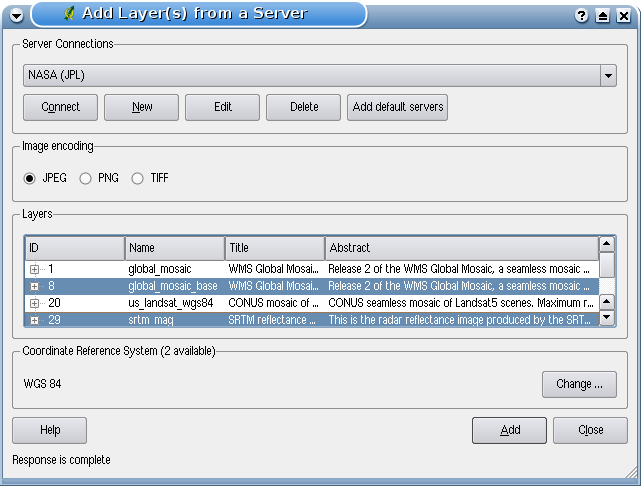
\includegraphics[clip=true,width=0.6\textwidth]{connection_wms}
\caption{Dialogue pour ajouter un serveur WMS, en indiquant ses couches
disponibles \nixcaption}\label{fig:connection_wms}
\end{figure}

% \begin{Tip}[ht]\caption{\textsc{Image Encoding}}
\begin{Tip}[ht]\caption{\textsc{Format d'image}}

% \qgistip{You will typically find that a WMS server offers you the choice
% of JPEG or PNG image encoding.  JPEG is a lossy compression format,
% whereas PNG faithfully reproduces the raw raster data.
Les serveurs WMS vous offriront typiquement le choix entre les formats d'image 
JPEG et PNG. JPEG est un format de compression avec perte, tandis que le format 
PNG reproduit pleinement les données raster brutes.

% Use JPEG if you expect the WMS data to be photographic in nature and/or you
% don't mind some loss in picture quality.  This trade-off typically reduces by
% 5 times the data transfer requirement compared to PNG.
Utilisez le format JPEG si vous pensez que la donnée WMS est une orthophotographie 
ou qu'une perte de qualité d'image ne vous pose pas de problème. Ce compromis 
vous permet de réduire par 5 le taux de transfert nécessaire comparé au  format PNG.

% Use PNG if you want precise representations of the original data, and you
% don't mind the increased data transfer requirements.
Utilisez le format PNG si vous désirez une représentation précise des données 
originales et que l'augmentation du taux de transfert ne vous pose pas de 
problème.\index{WMS!format d'image}
\end{Tip}

\minisec{Ordes des  couches} \label{ogc-wms-layers}

% The \tab{Layers} tab lists the layers available from the selected
% WMS server.  You may notice that some layers are expandible, this means
% that the layer can be displayed in a choice of image styles.
L'onglet \tab{Ordre des couches} liste les couches disponibles au sein du serveur 
WMS auquel vous êtes connectés. 
Vous remarquerez que certaines couches sont extensibles, cela signifie que 
la couche peut être affichée en fonction de plusieurs styles.

% You can select several layers at once, but only one image style per layer.
% When several layers are selected, they will be combined at the WMS Server
% and transmitted to \qg in one go.
Vous pouvez sélectionner plusieurs couches à la fois, mais seulement un style  d'image par couche. Lorsque plusieurs couches sont sélectionnées, celles-ci  seront combinées par le serveur WMS et transmises à \qg en une seule fois.

% \begin{Tip}[ht]\caption{\textsc{WMS Layer Ordering}}
\begin{Tip}[ht]\caption{\textsc{Ordonner les couches WMS}}
%In this version of QGIS, WMS layers rendered by a server are overlaid
%in the order listed in the Layers section, from top to bottom of the list.
%If you want to change the overlay order, you can use the \tab{Layer Order} tab. 
%\index{WMS!remote server!layer ordering}
%\end{Tip}

Dans cette version de \qg, les couches WMS créées par un serveur sont superposées dans le même ordre que celui listé dans la section des couches, du haut vers le bas de la liste. Si vous voulez modifier l'ordre des couches, vous pouvez alors utiliser le panneau \tab{Ordre des couches}.
\index{WMS!serveur distant!ordonner les couches}
\end{Tip}

\minisec{Transparence}\label{ogc-wms-transparency}

% In this version of \qg, the transparency setting is hard-coded to 
% be always on, where available.
Dans cette version de \qg, le paramètre de transparence est codé en dur pour  être toujours activé, si disponible.

% \begin{Tip}[ht]\caption{\textsc{WMS Layer Transparency}}
\begin{Tip}[ht]\caption{\textsc{Transparence des couches WMS}}
% \qgistip{The availability of WMS image transparency depends on
% the image encoding used:  PNG and GIF support transparency,
% whilst JPEG leaves it unsupported.
% \index{WMS!transparence de couche}
% }
La disponibilité de la transparence de l'image WMS dépend du format d'image utilisé : les formats PNG et GIF gèrent la transparence, tandis que le format JPEG ne le gère pas. \index{WMS!transparence de couche}
\end{Tip}

\minisec{Système de Référence de Coordonnées}
\index{WMS!CRS}
\index{WMS!coordinate reference system}
\index{OGC!coordinate reference system}
\index{Projections!WMS}
\index{Projections!CRS}
\index{Projections!système de référence de coordonnées}
\index{CRS}
\index{système de référence de coordonnées}
\index{SRS}
\index{Projections!SRS}

% A Coordinate Reference System (CRS) is the OGC terminology for a \qg
% Projection.
Un système de Référence de Coordonnées (CRS) est la terminologie de l'OGC pour
une projection \qg.

% Each WMS Layer can be presented in multiple CRSs, depending on the capability
% of the WMS server.  You may notice that the \textsl{x} changes in the
% \textsl{Coordinate Reference System (x available)} header as you select and
% deselect layers from the \tab{Layers} section.
Chaque couche WMS peut être représentée dans plusieurs projections (ou CRS), en fonction de la possibilité du serveur WMS. Vous pouvez avoir noté que les \textsl{x} changent dans l'en-tête du \textsl{Système de Référence des Coordonnées(x disponible)} lorsque vous sélectionnez et désélectionnez les couches de la section \tab{couches}.

% To choose a CRS, select \button{Change...} and a screen similar to
% Figure \ref{fig:projections} in Section \ref{label_projstart} will appear.
% The main difference with the WMS version of the screen is that only
% those CRSs supported by the WMS Server will be shown.
Pour choisir une projection, sélectionnez \button{Change\dots} et un dialogue similaire à la figure \ref{fig:projections} dans la section \ref{label_projstart} apparaitra. La principale différence avec l'écran de la version WMS est que seules les projections gérées par le serveur seront listées.

% \begin{Tip}[ht]\caption{\textsc{WMS Projections}}
\begin{Tip}[ht]\caption{\textsc{Les projections WMS}}
% \qgistip{For best results, make the WMS layer the first layer you add in the
% project.  This allows the project projection to inherit the CRS you used to
% render the WMS layer. On-the-fly projection (see
% Section \ref{sec:projection-specifying}) can then be used to fit any
% subsequent vector layers to the project projection. In this version of \qg,
% if you add a WMS layer later, and give it a different CRS to the current
% project projection, unpredictable results can occur.}
Pour de meilleurs résultats, faites en sorte que la couche WMS soit la première couche que vous ajoutez dans le projet. Cela permet à la projection du projet d'hériter la définition de la projection que vous avez utilisée pour le rendu de la couche WMS. La projection à la volée (voir Section \ref{sec:projection-specifying}) peut être utilisée pour placer les couches vectorielles supplémentaires dans la projection du projet. Dans cette version  de \qg, si vous ajoutez une couche WMS plus tard et lui donner une projection différente de celui du projet en cours, cela peut entraîner des résultats aléatoires.
\end{Tip}

% 
% server-search tab.
%
%\subsection{Server-Search}
%\label{sec:serversearch}
%\index{WMS!serversearch}
%\index{WMS!search}
%\index{OGC!search}
\subsection{Recherche de serveur}
\label{sec:serversearch}
\index{WMS!Recherche de serveur}
\index{WMS!chercher}
\index{OGC!chercher}

Dans \qg vous pouvez rechercher directement des serveurs WMS.  La figure \ref{fig:searchtab} montre le nouvel onglet \tab{Recherche de serveurs} avec la fenêtre \dialog{Ajouter des couches d'un serveur}.

\begin{figure}[ht]
  \begin{center}
	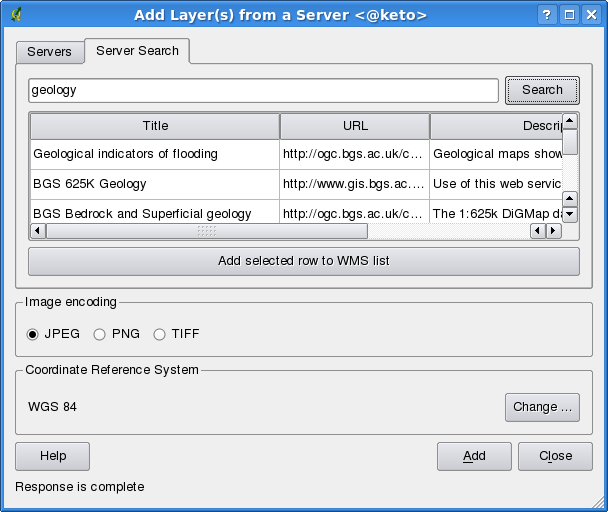
\includegraphics[clip=true,width=0.6\textwidth]{wms_server-search}
	\caption{Fenêtre pour rechercher des serveurs WMS avec des mots-clés \nixcaption}\label{fig:searchtab}
  \end{center}
\end{figure}

%As you can see it is possible to enter a search-string in the textfield an
%hit the \button{Search} button.
Comme vous pouvez le voir, il est possible d'entrer une chaîne de recherche dans un champ texte puis cliquez sur le bouton \button{Chercher}.
%After a short while the search result will be populated into the tab below
%the textfield. 
Après un court moment d'attente, le résultat de la recherche sera affiché dans l'onglet dessous le champ texte.
%Browse the result list and inspect your searchresults within the table. To
%visualize the results, select an table entry, press the \button{Add
%selected row to WMS-list} button and change back to the \tab{server} tab.
Naviguer dans la liste et inspecter vos résultats de la recherche dans le tableau. Pour visualiser le résultat, sélectionnez l'entrée du tableau, pressez le bouton \button{Ajoutez les lignes sélectionnées de la liste WMS} et retournez sur l'onglet \tab{serveur}.
%\qg automatically has updated your server list and the selected
%searchresult is already enabled in the list of saved WMS-servers.
\qg a automatiquement mis à jour votre liste de serveur et les résultats sélectionnés de la recherche sont déjà activés dans la liste des serveurs WMS sauvés.
%You only need to request the list of layers by clicking the
%\button{Connect} button.
Vous avez seulement besoin d'interroger la liste des couches en cliquant sur le bouton \button{Connecter}.
%This option is quite handy when you want to search maps by specific
%keywords.
Cette option est pratique quand vous voulez chercher des couches par des mots clés spécifiques.
%Basically this option is a frontend to the API of
%\url{http://geopole.org}.
Fondamentalement cette option est un frontend à l'API \url{http://geopole.org}.

% Layer Order
\subsection{Ordre des couches} \label{sec:layerorder}
\index{WMS!layerorder}

Dans l'onglet \tab{Ordre des couches} vous pouvez régler l'ordre d'affichage des couches sélectionnées.
Cela permet lorqu'on a sélectionné une liste de couches d'un serveur cartographique WMS et si vous voulez
 changer l'ordre d'affichage de certaines couches.

Sélectionner juste la couche que vous voulez changer et presser sur le bouton monter-descendre au-dessus de la liste des couches.

%\subsection{Tilesets}\label{sec:tilesets}
\subsection{Jeux de Tuiles}\label{sec:tilesets}
\index{WMS!tileset}
\index{WMS!WMS-C}

%When using WMS-C (Cached WMS) Services like
%\url{http://labs.metacarta.com/wms-c/Basic.py} you are able to browse
%through the \tab{tiles}-tab given by the server. Additional information like
%tilesize, formats and supported CRS are listed in this table.
Lorsque vous utilisez un service WMS-C (Cache WMS) tel que \url{http://labs.metacarta.com/wms-c/Basic.py}, vous pouvez parcourir le panneau \tab{Jeux de Tuile} concernant le serveur. Des informations telles que la taille des tuilles, leurs formats et les SCR supportés sont affichées.

%In combination with this feature you can use the tile scale slider from
%the \mainmenuopt{View}>\dropmenuopt{tile scale slider}, which gives you
%the available scales from the tileserver with nice slider docked in.
Vous disposez également d'une barre de zoom depuis \mainmenuopt{Vue}>\dropmenuopt{Barre d'échelle des tuiles}, il vous permet de faire défiler les différents niveaux de tuiles disponibles sur le serveur.

% \subsection{Using the Identify Tool}\label{sec:ogc-wms-identify}
\subsection{Utiliser l'outil Identifier}\label{sec:ogc-wms-identify}
\index{WMS!identifier}
\index{identifier!WMS}
\index{WMS!GetFeatureInfo}

% Once you have added a WMS server, and if any layer from a WMS server is
% queryable, you can then use the \toolbtntwo{mActionIdentify}{Identify} tool to
% select a pixel on the map canvas. A query is made to the WMS server for each
% selection made.
Une fois que vous avez ajouté un serveur WMS et si une couche du serveur WMS est interrogeable, vous pouvez utiliser l'outil  \toolbtntwo{mActionIdentify}{Identifier} pour sélectionner un pixel sur la carte. Une requête est envoyée au serveur WMS pour chaque sélection effectuée.

% The results of the query are returned in plain text. The formatting of this
% text is dependent on the particular WMS server used.
Les résultats de la requête sont renvoyés au format texte. Le formatage de ce texte est dépendant du serveur WMS utilisé.

% \subsection{Viewing Properties}
\subsection{Visualiser les propriétés}
\label{sec:ogc-wms-properties}\index{WMS!propriétés}
\index{rasters!propriétés}

% Once you have added a WMS server, you can view its properties by
% right-clicking on it in the legend, and selecting \button{Properties}.
Une fois que vous avez ajouté un serveur WMS, vous pouvez voir ses propriétés en cliquant avec le bouton droit de la souris sur sa légende, et en sélectionnant le bouton  \button{Propriétés}.

% \minisec{Metadata Tab}\label{sec:ogc-wms-properties-metadata}
\minisec{Onglet métadonnées}\label{sec:ogc-wms-properties-metadata}
\index{rasters!métadonnées}
\index{WMS!métadonnées}
\index{WMS!possibilités}

% The \tab{Metadata} tab displays a wealth of information about the WMS server,
% generally collected from the Capabilities statement returned from that server.
L'onglet \tab{métadonnées} affiche la richesse des informations du serveur WMS, généralement collecté à partir de la requête Capabilities renvoyée par le serveur.

% Many definitions can be gleaned by reading the WMS standards
% \cite{OGCWMS010101web}, \cite{OGCWMS010300web}, but here are a few handy
% definitions:
Beaucoup de définitions peuvent être obtenues par la lecture des normes WMS \cite{OGCWMS010101web}, \cite{OGCWMS010300web}, mais en voici quelques-unes :

\begin{itemize}[label=--]
% \item \textbf{Server Properties}
\item \textbf{Propriétés du serveur}

\begin{description}
% \item[WMS Version :]  The WMS version supported by the server.
\item[Version du WMS :] la version du serveur WMS géré par le serveur.

% \item[Image Formats}    — The list of MIME-types the server can
% respond with when drawing the map.  \qg supports whatever formats the
% underlying Qt libraries were built with, which is typically at least
% \texttt{image/png} and \texttt{image/jpeg}.
\item[Formats d'image :]  la liste des types MIME que le serveur peut renvoyer lors qu'il dessine la carte. \qg gère tous les formats pour lesquelles la bibliothèque Qt en sous-couche a été compilée, qui est typiquement à minima les types \texttt{image/png} et \texttt{image/jpeg}.

% \item[Identity Formats :]  The list of MIME-types the server can
% respond with when you use the Identify tool.  Currently \qg supports the
% \texttt{text-plain} type.
\item[Formats de l'outil Identitier :]  la liste des types MIME auxquels le serveur peut répondre quand vous utilisez l'outil Identifier. Pour l'instant \qg gère le type \texttt{text-plain}.
\end{description}

% \item[Layer Properties}
\item \textbf{Propriétés de la couche}

\begin{description}
% \item[Selected}         — Whether or not this layer was selected when
% its server was added to this project.
\item[Selectionné :]  si cette couche a été sélectionnée ou pas quand son serveur a été ajouté au projet.

% \item[Visible}          — Whether or not this layer is selected as
% visible in the legend.  (Not yet used in this version of \qg.)
\item[Visible :]  si cette couche a été sélectionnée ou non comme visible dans la légende (pas encore utilisé dans cette version de \qg).

% \item[Can Identify}     — Whether or not this layer will return any
% results when the Identify tool is used on it.
\item[Peut identifier :]  si cette couche retournera ou pas des résultats quand l'outil Identifier est utilisé sur celle-ci.

% \item[Can be Transparent} - Whether or not this layer can be rendered
% with transparency. This version of \qg will always use transparency if this is
% \textsl{Yes} and the image encoding supports transparency
\item[Peut être transparent :]  si cette couche peut être rendue ou non avec une transparence. Cette version de \qg utilisera toujours la transparence si cette option est à \textsl{Oui} et que le format d'image gère la transparence.
% BM: doesn't seem to work?
%                                    (see Section
%                                    \ref{ogc-wms-transparency}
%                                    ).
% \item[Can Zoom In}      — Whether or not this layer can be zoomed in
% by the server.  This version of \qg assumes all WMS layers have this set
% to \textsl{Yes}. Deficient layers may be rendered strangely.
\item[Peut zoomer :]  si on peut zoomer ou non sur cette couche avec le serveur. Cette version de \qg assume que toutes les couches WMS ont ce paramètre défini à \textsl{Oui}. Les couches déficientes peuvent être rendues d'une manière étrange.

% \item[Cascade Count}    — WMS servers can act as a proxy to other WMS
% servers to get the raster data for a layer.  This entry shows
% how many times the request for this layer is forwarded to peer WMS servers for
% a result.
\item[Décompte des cascades :]  les serveurs WMS peuvent agir comme un proxy à d'autres serveurs WMS pour obtenir des données pour une couche. Cette entrée affiche le nombre de fois où la requête pour cette couche est redirigée vers un autre serveur WMS pour un résultat.

% \item[Fixed Width}, \textbf{Fixed Height}     — Whether or not this
% layer has fixed source pixel dimensions. This version of \qg assumes all WMS
% layers have this set to nothing. Deficient layers may be rendered strangely.
\item[Largeur fixe, hauteur fixe :]  si une couche a des dimensions du pixel source limitées. Cette version de \qg suppose que toutes les couches WMS ont ce paramètre fixé. Les couches déficientes peuvent être rendues d'une manière étrange.

% \item[WGS 84 Bounding Box :]  The bounding box of the layer, in WGS 84
% coordinates. Some WMS servers do not set this correctly (e.g. UTM coordinates
% are used instead).  If this is the case, then the initial view of this layer
% may be rendered with a very ``zoomed-out'' appearance by \qg. The WMS
% webmaster should be informed of this error, which they may know as the WMS XML
% elements \texttt{LatLonBoundingBox}, \texttt{EX\_GeographicBoundingBox} or the
% CRS:84 \texttt{BoundingBox}.
\item[Limite du contour en WGS 84 :]  la limite du contour de la couche, en coordonnées WGS 84. Certains serveurs WMS ne définissent pas ceci correctement (par exemple, des coordonnées UTM sont utilisées à la place). Si cela est le cas, alors la vue initiale sera rendue avec une vue très étendue. Le webmaster du WMS doit être informé de cette erreur, qui sont connu en tant qu'éléments XML \texttt{LatLonBoundingBox}, \texttt{EX\_GeographicBoundingBox} ou \texttt{BoundingBox} CRS:84 du WMS.

% \item[Available in CRS :]  The projections that this layer can be
% rendered in by the WMS server. These are listed in the WMS-native format.
\item[Disponibilité des CRS :]  les projections que l'on peut utiliser par le serveur WMS. Ceux-ci sont listés dans le format natif du WMS.

% \item[Available in style :]  The image styles that this layer can be
% rendered in by the WMS server.
\item[Disponibilité des styles :]  les styles des images de cette couche qui peuvent être utilisés pour le rendu par le serveur WMS.

\end{description}

\end{itemize}


% \subsection{WMS Client
% Limitations}\label{sec:ogc-wms-limits}\index{WMS!client!limits}
\subsection{Limitations du client
WMS}\label{sec:ogc-wms-limits}\index{WMS!client!limites}

% Not all possible WMS Client functionality had been included in this version of
% \qg. Some of the more notable exceptions follow:
Seules quelques fonctionnalités du client WMS ont été incluses dans cette version de \qg. Les exceptions les plus notables sont présentées ci-après :

% \minisec{Editing WMS Layer Settings}
\minisec{Éditer la configuration d'une couche WMS}
\index{WMS!configuration des couches!édition}

% Once you've completed the \toolbtntwo{mActionAddWmsLayer}{Add WMS layer}
% procedure, there is no ability to change the settings.
Une fois que vous avez complété la procédure d' \toolbtntwo{mActionAddWmsLayer}{Ajout de couches WMS}, il n'y aucun moyen de modifier la configuration.

% A workaround is to delete the layer completely and start again.
Une solution de contournement est de supprimer la couche et de recommencer.

% \minisec{WMS Servers Requiring Authentication}
\minisec{Serveurs WMS nécessitant une authentification}
\index{WMS!serveur distant!authentication}
\index{WMS!serveur distant!basic authentification}

% Only public WMS servers are accessible.
% There is no ability to apply a user name and password combination
% as an authentication to the WMS server.
Seuls les serveurs WMS publics sont accessibles. Il n'y a pas de possibilités pour appliquer une combinaison nom d'utilisateur et mot de passe comme authentification à un serveur WMS. Pour l'instant, les services WMS publics accessibles et sécurisés sont gérés. Les serveurs WMS sécurisés peuvent être interrogés par une authentification publique. Vous pouvez  ajouter les paramètres d'identification (optionnel) quand vous ajoutez un serveur WMS. Voir la section  \ref{sec:ogc-wms-servers} pour les détails.


% \begin{Tip}[ht]\caption{\textsc{Accessing secured OGC-layers}}
\begin{Tip}[ht]\caption{\textsc{Accéder des couches OGC sécurisées}}
% \qgistip{If you need to access secured layers, you could use InteProxy as
% a transparent proxy, which does supports several authentification methods.
% More information can be found at the InteProxy-manual found on the website
% \url{http://inteproxy.wald.intevation.org}.
Si vous avez besoin d'accéder à des couches sécurisées avec d'autres méthodes sécurisés que des authentifications basiques, vous pouvez utiliser InteProxy comme proxy transparent, qui gère plusieurs méthodes d'authentification. Vous pouvez trouver plus d'informations dans le manuel InteProxy que vous pouvez trouver sur le site \url{http://inteproxy.wald.intevation.org}. \index{WMS!couches sécurisées!}\index{OGC!Authentication}
\end{Tip}

\begin{Tip}[ht]\caption{\textsc{QGIS WMS Mapserver}}
%Note that with the Version 1.7.0 QGIS brings its own implementation of a
%WMS 1.3.0 Mapserver. Read more about this at chapter
%\ref{label_qgismapserver}.
%\index{WMS!QGISmapserver}\index{OGC!WMS1.3.0}
Notez que la version 1.7.0 QGIS apporte sa propre implémentation d'un WMS 1.3.0 Mapserver.
Lisez en plus au chapitre \ref{label_qgismapserver}.
\index{WMS!QGISmapserver}\index{OGC!WMS1.3.0}
\end{Tip}

% \section{WFS Client}
\section{Client WFS/WFS-T}\label{sec:ogc-wfs}
 \index{WFS!WFS-T}
 \index{WFS!Transactionnel}

% In QGIS, a WFS layer behaves pretty much like any other vector layer. You
% can identify and select features and view the attribute table. Since QGIS 1.6 
% editing (WFS-T) is also supported, if the server provides this feature. To start 
% the WFS plugin you need to open \mainmenuopt{Plugins} \arrow 
% \dropmenuopttwo{mActionShowPluginManager}{Plugin Manager...}, activate the 
% \checkbox{WFS plugin} checkbox and click \button{OK}.

Dans \qg, une couche WFS se comporte à peu près comme n'importe quelle autre couche vecteur. Vous pouvez identifier et sélectionner des objets et voir la table attributaire. Depuis QGIS 1.6, l'édition est prise en charge si le serveur le propose. Pour lancer l'extension WFS, vous avez besoin d'ouvrir des \mainmenuopt{Extensions} > \dropmenuopttwo{mActionShowPluginManager}{Gestionnaire d'extension ...}, activez l'extension \checkbox{WFS} et cliquez sur le bouton \button{OK}.

% A new \toolbtntwo{mIconAddWfsLayer}{Add WFS Layer} icon appears next 
% to the WMS icon. Click on it to open the dialog. In General adding a WFS 
% layer is very similar to the procedure used with WMS. The difference is 
% there are no default servers defined, so we have to add our own.
Une nouvelle icône \toolbtntwo{mIconAddWfsLayer.png}{Ajouter une couche WFS} apparaît à côté de celle du WMS. Cliquez dessus pour ouvrir la boîte de dialogue. En général ajouter une couche WFS est identique à la procédure utilisée pour une couche WMS. La différence est qu'il n'y a pas de serveurs par défaut, vous devez donc en ajouter.

% \subsection{Loading a WFS Layer}
\subsection{Charger une couche WFS}

% As an example we use the DM Solutions WFS server and display a layer. The URL
% is:
Comme exemple, nous utilisons le serveur WFS de DM Solutions et affichons une
couche. L'URL est :
\begin{verbatim}
http://www2.dmsolutions.ca/cgi-bin/mswfs_gmap?VERSION=1.0.0&SERVICE=
wfs&REQUEST=GetCapabilities
\end{verbatim}

\begin{enumerate}
%   \item Make sure the WFS plugin is loaded; if not, open the Plugin Manager and
% load it
  \item Assurez-vous que l'extension WFS est activée ; si ce n'est pas le cas, ouvrez le gestionnaire d'extensionset activez le.
%   \item Click on the \toolbtntwo{mIconAddWfsLayer}{Add WFS Layer} tool on the
% plugins toolbar
  \item Cliquez sur le bouton \toolbtntwo{mIconAddWfsLayer}{Ajoutez une couche WFS} dans la boîte à outil des plugins.
%   \item Click on \button{New} 
  \item Cliquez sur \button{Nouveau} 
%   \item Enter \inputtext{Name}{DM Solutions} as the name
  \item Entrez \inputtext{Nom}{DM Solutions} comme nom.
%   \item Enter the URL (see previous page)
\item Entrez l'URL (voir page précédente).
%   \item Click \button{OK}
\item Cliquez sur \button{OK}
%   \item Choose \selectstring{Server Connections}{DM Solutions} from the
% drop-down box
  \item Choisissez \selectstring{Connexions au serveur}{DM Solutions} dans la liste déroulante.
%   \item Click \button{Connect}
\item Cliquez sur \button{Connecter}.
%   \item Wait for the list of layers to be populated
\item Attendez que la liste des couches soit complètes.
%   \item Click on the \clicklistitem{Canadian Land} layer
\item Cliquez sur la couche\clicklistitem{Canadian Land}.
%   \item Click \button{Ok} to add the layer to the map
\item Cliquez sur \button{Ok} pour ajouter la couche à la carte.
%   \item Wait patiently for the features to appear
\item Patientez que les objets apparaissent.
\end{enumerate}

Notez que l'extension WFS reconnait également les paramètres proxy que vous avez définis dans vos préférences.

\begin{figure}[ht]
    \centering
    \caption{Ajoutez une couche WFS \nixcaption}\label{fig:wfs_dmsolutions}
    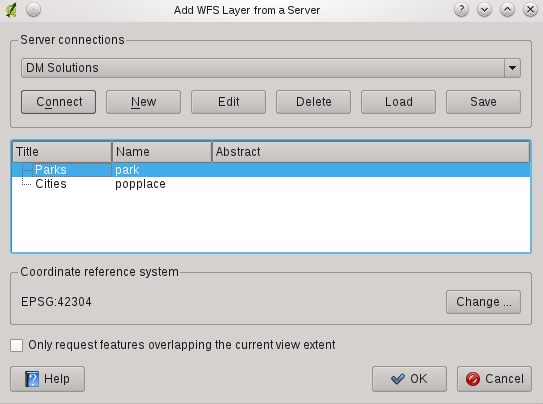
\includegraphics[clip=true, width=8cm]{connection_wfs}
\end{figure}


%Without using the checkbox \checkbox{Only request features overlapping the
%current view extent} QGIS fetches all features from the WFS-server. If you
%only want to have a small selection based on your extent, zoom to the area
%of interest, request the WFS-layer again and make sure you have checked
%the checkbox mentioned above. Basically this addes the BBOX-parameter with
%the values from you current extent to the WFS-query. This is extremly
%usefull when you only want to request \textbf{some} features from a huge
%WFS-dataset.

Si la case \checkbox{Demander uniquement les entités dépassant l'étendue de la vue actuelle} n'est pas cochée, alors \qg récupére l'ensemble des entités du serveur WFS. Cochez la si vous désirez uniquement une petite sélection basée sur l'emprise de votre carte, cela rajoute la paramètre BBOX qui indique dans la requête l'étendue des données à récupérer. C'est très pratique lorsque vous voulez seulement quelques entités d'un énorme jeu de données WFS.

% You'll notice the download progress is visualized in the left bottom of the
% \qg main window. 
% Once the layer is loaded, you can identify and select a province or two and
% view the attribute table.
Vous remarquerez que la progression du téléchargement est affichée en bas à
gauche de la fenêtre principale de \qg.
% \begin{Tip}[ht]\caption{\textsc{Finding WMS and WFS Servers}}
\begin{Tip}[htb]\caption{\textsc{Trouver des serveurs WMS et WFS}}
% \qgistip{You can find additional WMS and WFS servers by using Google or your
% favorite search engine. There are a number of lists with public URLs, some 
% of them maintained and some not.
Vous pouvez trouver des serveurs WMS et WFS supplémentaires en utilisant Google ou votre moteur de recherche préféré. Il y a un certain nombre de sites qui listent des URL publiques, certaines maintenues d'autres non. \index{WFS!serveur distant!}
\end{Tip}
% Remember this plugin works best with UMN MapServer WFS servers. It still
% could be, that you might experience random behavior and crashes. You can look
% forward to improvements in a future version of the plugin.
Souvenez-vous que les extensions fonctionnent mieux avec des serveurs WFS sous MapServer. Il est encore possible que vous ayez à faire face à quelques problèmes et crashes. Vous pouvez vous attendre à des améliorations dans les versions futures de l'extension.

Cela signifie que seule la version 1.0.0 des WFS est gérée. À ce point il n'y a pas eu de test pour les autres versions des services WFS des serveurs WFS.
Si vous rencontrez des problèmes avec d'autres serveurs WFS, s'il vous plait n'hésitez  pas à contacter l'équipe de développement. Référez-vous à la section  \ref{label_helpsupport} pour plus d'information sur les listes de diffusions.

%\begin{Tip}[ht]\caption{\textsc{Accessing secure WFS Servers}}
%\qgistip{
%Within the dialog \dialog{Create a new WFS-connection} accidentily
%described \qg does not support authenficated WFS-connections yet. Within
%one of the next releases we expect to also support authenticated
%WFS-servers. Meanwhile you could use InteProxy
%(\url{http://inteproxy.wald.intevation.org}) for accessing authenticated
%WFS-servers.
%\index{WFS!authenticate remote server!}
%\index{WFS!secured WFS server!}
%}
%\end{Tip} 

%\begin{Tip}[htb]\caption{\textsc{Interoger des serveurs WFS sécurisés}}
%Dans la fenêtre \dialog{Créer une nouvelle connexion WFS} accidentellement décrite \qg ne gère pas les connexions WFS authentifiées pour le moment. Dans les prochaines versions, nous %espérons gérer les serveurs WFS authentifiés. Pour l'instant, vous pouvez utiliser  InteProxy (\url{http://inteproxy.wald.intevation.org}) pour interroger les serveurs WFS authentifiés.
%\index{WFS!authentification serveur distant!}
%\index{WFS!serveur WFS sécurisé!}
%\end{Tip} 